% !TEX TS-program = pdflatex
% !TEX encoding = UTF-8 Unicode
% !TEX root = ../main.tex
% !TEX spellcheck = en-US
% ****************************************************************************************
% File: solver_comparison.tex
% Author:  Schmid 
% Date: 
% ****************************************************************************************
\chapter{Comparison of linear and turbulent model}
\label{chapter:solver_comp}

While solving a problem in the fluent domain it is necessary to choose a valid model. We could either use a linear model or a turbulent model.
This chapter deals with the comparison of a linear model, a turbulent k-omega (SST) model, a turbulent k-epsilon model and a turbulent k-kl-epsilon model.


The laminar and k-omega model can be applied without further investigation of the y+ value. The y+ value quantifies the interaction between turbulence and the wall, therefore it is not applicable to a laminar model. The k-omega model uses enhanced wall treatment, therefore it is a 2-layer model which is not sensitive to the y+ value.
For the k-epsilon model we also applied enhanced wall treatment but due to the properties of the model we looked into the y+ value. The k-kl-omega model was applied with standard configuration and the y+ value was also investigated. Figure \ref{fig:k_epsilon_enhanced_y_plus} shows the critical region of the geometry with the plotted y+ values for k-epsilon model. The y+ values differes depending on the position and the critical length, the figure shows that the value is largely way below 1 and only is close to 1 at positions where you would expect the biggest influence of the wall to the (turbulent) flow.
The same applies to the y+ values for the k-kl-omega model as displayed in figure \ref{fig:k_kl_omega_y_plus}.

\begin{figure}[htbp]   
    \centering
    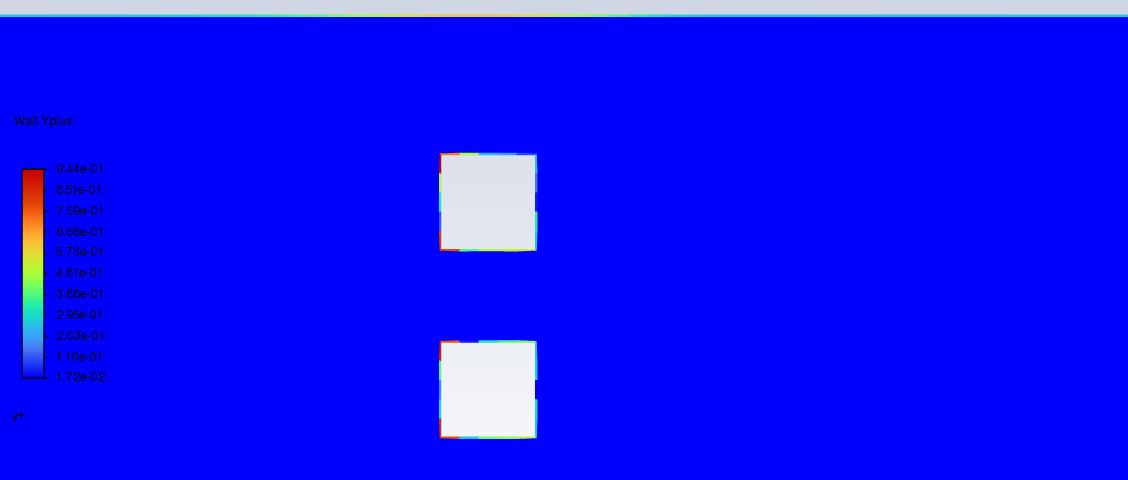
\includegraphics[width=0.8\textwidth]{img/y_plus_k_epsilon_enhanced_wt.png}
    \caption{y+ plot for k-epsilon with enhanced wall treatment}
    \label{fig:k_epsilon_enhanced_y_plus}
\end{figure}

\begin{figure}[htbp]   
    \centering
    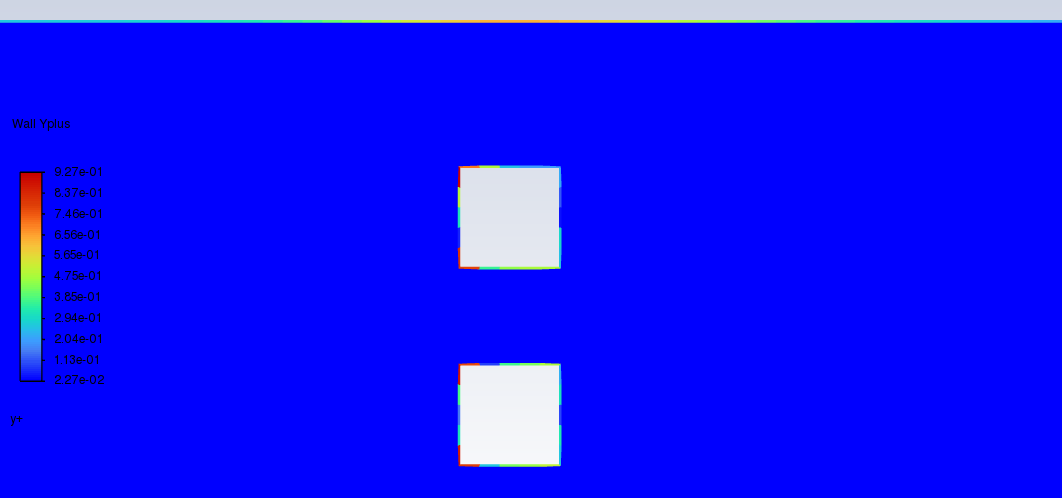
\includegraphics[width=0.8\textwidth]{img/y_plus_k_kl_omega_detail_inf5.png}
    \caption{y+ plot for k-kl-omega}
    \label{fig:k_kl_omega_y_plus}
\end{figure}

For the comparison the basic geometry is used, the meshing is done according to the results of chapter \ref{chapter:meshing}.
To compare the results the velocity, pressure and temperature is plotted.

\paragraph{Temperature Plot}~

Plotting the static temperature for all 4 models results in a temperature distribution as seen in figure \ref{fig:temp_plot}.
The plot contains all four models for easier comparison, every window in the plot is labeled with the used model. 
The laminar model offers the least symmetrical result, however a more or less symmetrical result would be expected with our basic geometry.
The laminar model seems to introduce eddies that affect the flow and the temperature distribution resulting in a unsymmetrical distribution.

The k-epsilon model with enhanced wall treatment has a sudden transition in temperature right after the fluid passed the heater. However, the temperature at the outlet is the same as with the other models, even tho the distribution (average over outlet) is lower.

The k-omega and k-kl-omega models both offer a good result. The k-kl-omega model however uses more equations and therefore introduces more computational effort and should be used for problems with a flow in the transition state between laminar and turbulent flow.
The result of the k-omega model is credible.

\begin{figure}[htbp]   
    \centering
    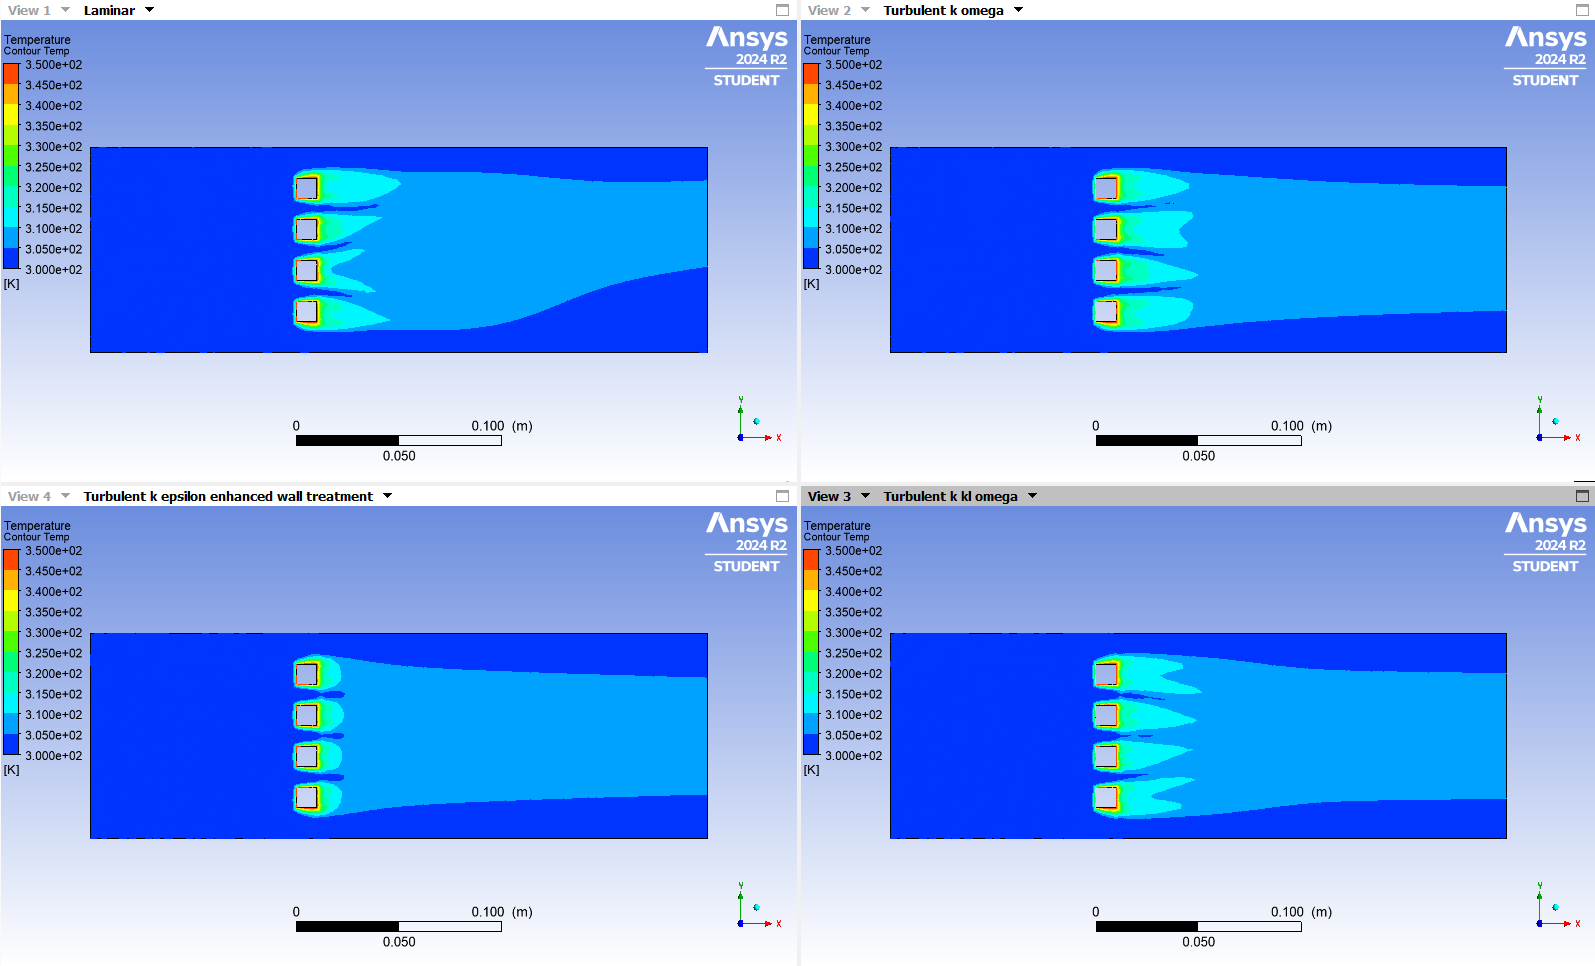
\includegraphics[width=1\textwidth]{img/Temp_plot_comparison.png}
    \caption{Temperature plot for all 4 models}
    \label{fig:temp_plot}
\end{figure}

\paragraph{Velocity Plot}~

The velocity plot supports the observations from the temperature plot.
Especially for the k-epsilon model the nearly nonexistent difference in velocity due to the heater seems suspicious. 
The 


\begin{figure}[htbp]   
    \centering
    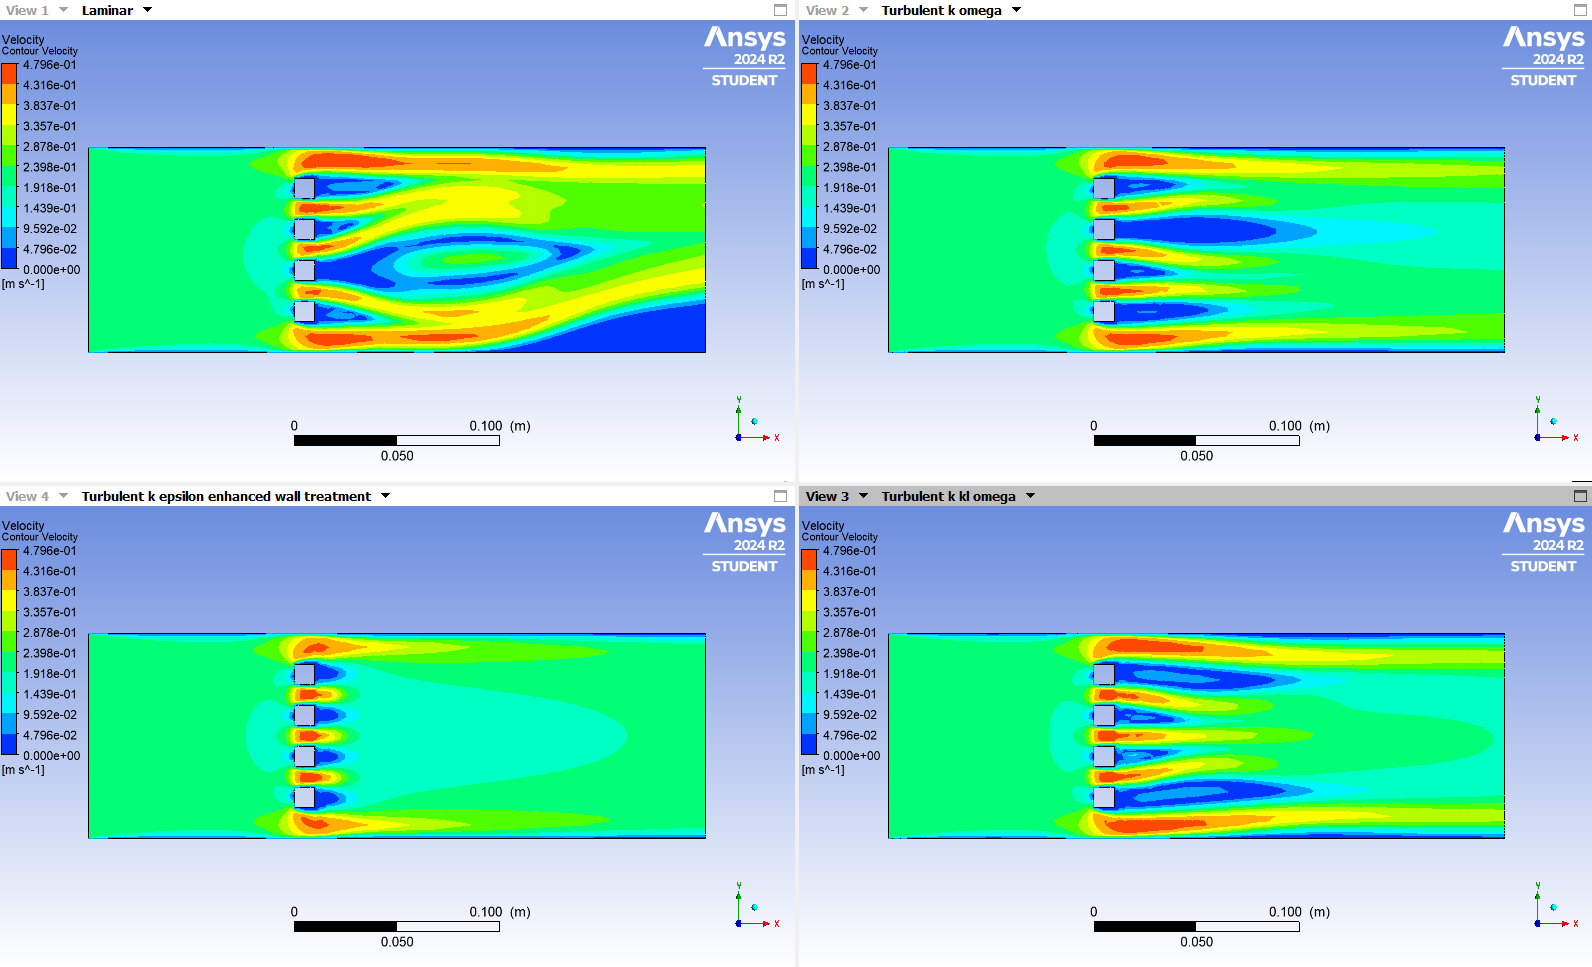
\includegraphics[width=1\textwidth]{img/Velocity_plot_comparison.png}
    \caption{Velocity plot for all 4 models}
    \label{fig:velocity_plot}
\end{figure}

\paragraph{Pressure Plot}~

\begin{figure}[htbp]   
    \centering
    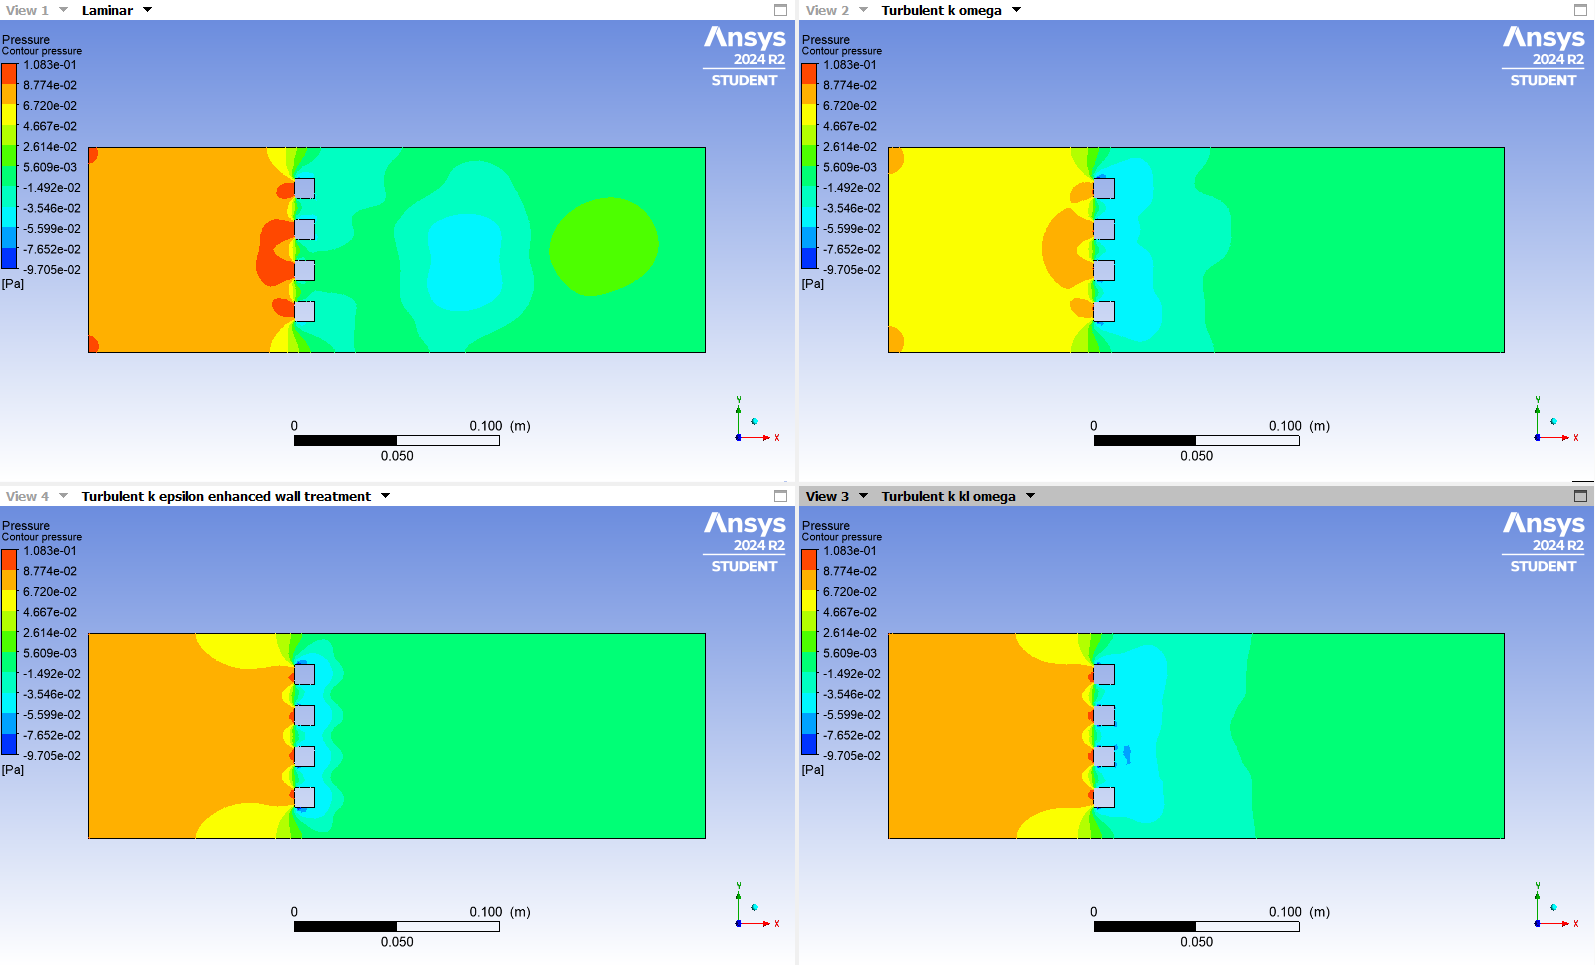
\includegraphics[width=1\textwidth]{img/Pressure_plot_comparison.png}
    \caption{Pressure plot for all 4 models}
    \label{fig:press_plot}
\end{figure}

% EOF